This layer allows access for data web based clients. Clients connect to the gateway to request resources. If the request passes the authentication, it will be sent to the core.

\begin{figure}[h!]
	\centering
 	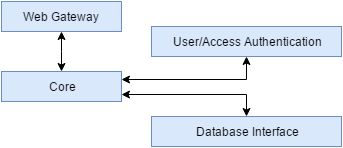
\includegraphics[width=0.60\textwidth]{images/web_service_layer}
 \caption{Example subsystem description diagram}
\end{figure}

\subsection{Web Gateway}
Web Gateway is a html controller that parses the html request.

\subsubsection{Assumptions}
The Web Gateway subsystem makes the assumption that any improperly formatted html request will be ignored.

\subsubsection{Responsibilities}
Web Gateway should parse the html request.

\subsubsection{Subsystem Interfaces}

\begin {table}[H]
\caption {Subsystem interfaces} 
\begin{center}
    \begin{tabular}{ | p{1cm} | p{6cm} | p{3cm} | p{3cm} |}
    \hline
    ID & Description & Inputs & Outputs \\ \hline
    \#01 & HTML Interface & \pbox{3cm}{HTML Requests} & \pbox{3cm}{JSON Objects}  \\ \hline
    \#02 & Database Interface & \pbox{3cm}{JSON Objects} & \pbox{3cm}{JSON Objects}  \\ \hline
    \end{tabular}
\end{center}
\end{table}

\subsection{User/Access Authentication}
User/Access Authentication validates the html request based on the tokens.

\subsubsection{Assumptions}
The User/Access Authentication subsystem makes the assumption that any unauthorized html tokens will be ignored.

\subsubsection{Responsibilities}
User/Access Authentication should check the html request for its validity. 

\subsubsection{Subsystem Interfaces}

\begin {table}[H]
\caption {Subsystem interfaces} 
\begin{center}
    \begin{tabular}{ | p{1cm} | p{6cm} | p{3cm} | p{3cm} |}
    \hline
    ID & Description & Inputs & Outputs \\ \hline
    \#01 & HTML Interface & \pbox{3cm}{HTML Requests} & \pbox{3cm}{JSON Objects}  \\ \hline
    \#02 & Database Interface & \pbox{3cm}{JSON Objects} & \pbox{3cm}{JSON Objects}  \\ \hline
    \end{tabular}
\end{center}
\end{table}

\subsection{Database Interface}
Database Interface helps connect the core to the actual database to fetch and store the data in the actual database.

\subsubsection{Assumptions}
The database Interface subsystem makes the assumption that the data passing through it is in the final form so that it can be stored in the actual database.

\subsubsection{Responsibilities}
The database Interface should allow the data to pass to the Database Layer. Invalid data should be buffered within the subsystem before passing it to the Database Layer.

\subsubsection{Subsystem Interfaces}

\begin {table}[H]
\caption {Subsystem interfaces} 
\begin{center}
    \begin{tabular}{ | p{1cm} | p{6cm} | p{3cm} | p{3cm} |}
    \hline
    ID & Description & Inputs & Outputs \\ \hline
    \#01 & Database Interface & \pbox{3cm}{JSON Objects} & \pbox{3cm}{JSON Objects}  \\ \hline
    \end{tabular}
\end{center}
\end{table}

\subsection{Core}
The Web Service Layer Core subsystem will distribute all the parsed html requests to the appropriate layer in the total system.

\subsubsection{Assumptions}
Core subsystem makes the assumption that there would be some subsystem that would take care of the distributed parsed requests.

\subsubsection{Responsibilities}
The core subsystem should make sure to distribute the parsed html requests to the appropriate subsystem.

\subsubsection{Subsystem Interfaces}

\begin {table}[H]
\caption {Subsystem interfaces} 
\begin{center}
    \begin{tabular}{ | p{1cm} | p{6cm} | p{3cm} | p{3cm} |}
    \hline
    ID & Description & Inputs & Outputs \\ \hline
    \#01 & HTML Interface & \pbox{3cm}{HTML Requests} & \pbox{3cm}{JSON Objects}  \\ \hline
    \#02 & Database Interface & \pbox{3cm}{JSON Objects} & \pbox{3cm}{JSON Objects}  \\ \hline
    \end{tabular}
\end{center}
\end{table}